\section{Auto-completion and Abbreviations}
\label{section:abbrevs}

Even though the user can easily manipulate Unicode symbols after we implemented the Isabelle file-system, it is still hard to input them. Most users do not have keyboards made for writing mathematical notation. That is why, we need to define ways in which the user can input such symbols.

There are two ways this is achieved:
\begin{itemize}
    \item\textbf{Auto-completion.} While the user is writing the latex notation for the symbol, a dialog pops up with the matching symbol. When the user selects one of these options the text is then replaced by the respective symbol.
    \item\textbf{Abbreviations.} Instead of writing the whole latex notation for a symbol, the user can use one of the preconfigured abbreviations. This abbreviation gets then replaced with the respective symbol. For example the abbreviation \texttt{\textendash\textendash>} would get replaced by the symbol $\rightarrow$.
\end{itemize}

\paragraph{Current Implementation.}
Both abbreviations and auto-completion are implemented in jEdit. In VSCode abbreviations are not implemented. Auto-completion is already supported but only for completing the latex notation, not replacing it with the appropriate symbol. The difference between the auto-completions is illustrated below in \autoref{fig:auto-complete-example}.

\begin{figure}[!tbp]
    \centering
    \subfloat[][Auto-completion example in jEdit.]{
        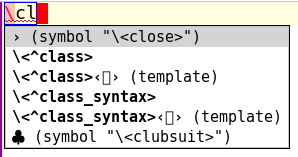
\includegraphics[width=0.4\textwidth]{figures/problem3/jedit_autocomplete.png}
    }
    \hfill
    \subfloat[][Auto-completion example in VSCode.]{
        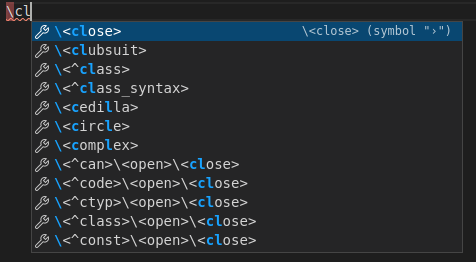
\includegraphics[width=0.55\textwidth]{figures/problem3/vscode_old_autocomplete.png}
    }
    \caption{Example comparison of auto-completion between jEdit and VSCode.}
    \label{fig:auto-complete-example}
\end{figure}

\paragraph{Solutions.}
The auto-completion can be easily configured to replace the latex notation with the symbol. The notation should still be in the label of the completion, or else it wouldn't be searchable.

The abbreviations need to be implemented in the front-end, for this reason we first need to extend the symbols endpoint to include the abbreviations for each symbol. Many of these abbreviations are not unique, i.e. they are not assigned to just one symbol. For example \texttt{<{}<} is an abbreviation for $\langle$ and \texttt{<<}. These abbreviations will not be automatically replaced, but the auto-completion will show the different options as suggestions. Single character abbreviations are also handled by the auto-completion. Only unique abbreviations will be automatically replaced.

To make it more customizable, we let the user choose in the extension settings when abbreviations will be replaced. With the options being:
\begin{itemize}
    \item\textbf{none} Replacements are deactivated. No replacements are done.
    \item\textbf{non-alpha} Replaces all unique abbreviations that contain no alpha-numeric characters. (Abbrevitions such as \texttt{Un} for $\cup$ will not be replaced.) This is the default setting. 
    \item\textbf{all} Replaces all unique abbreviations.
\end{itemize}

After we have identified all unique abbreviations, we save them all these in a prefix tree so that they are efficiently searchable. We will use the same prefix tree class that we used in the Isabelle file system. The type of the prefix tree needs to be changed to accept not only number arrays but also strings. The key for the tree nodes will also be \texttt{number} or \texttt{string}, because there is no \texttt{char} type in TypeScript. Abbreviations that are prefixes of other abbreviations are saved with a space in the end. 

We also register a function that triggers when a text document is changed (i.e. user typing). It checks starting from the last typed character, backwards, if the text written is an abbreviation. For this reason we save the abbreviations in the prefix tree reversed. The text being typed is then replaced with the longest matching abbreviation. To also support multi-cursor abbreviation replacement, we start from the last edited part of the text. Doing this helps with keeping the ranges consistent for all different parts of the text document that were changed.

One problem that emerges from using this method is that using Undo after an abbreviation has been replaced doesn't work. When the user undoes an abbreviation replacement, a \texttt{TextChange} event is emitted which in turn triggers our function that ends up replacing the abbreviation again. This is solved by not triggering our function for \texttt{TextChange} events that are replacing one character. These kind of events are the undo events, where the user replaces the symbol with the abbreviation text.

\paragraph{Results.}
The input of Unicode symbols has been highly facilitated. Now the user can input symbols through auto-completion of latex notations and through abbreviations, as shown below in \autoref{fig:auto-complete-new} and \autoref{fig:auto-complete-new-abbrev}. Abbreviation replacement is almost instantaneous and the auto-completion suggestion box is also relatively fast. The user can also choose through the settings what level of abbreviation replacement he wants.

\begin{figure}[htbp]
    \centering
    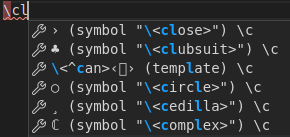
\includegraphics[width=0.7\textwidth]{figures/problem3/vscode_new_autocomplete.png}
    \caption{Example of latex notation auto-completion in VSCode.}
    \label{fig:auto-complete-new}
\end{figure}

\begin{figure}[htbp]
    \centering
    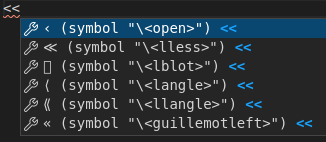
\includegraphics[width=0.7\textwidth]{figures/problem3/vscode_abbreviation_autocomplete.png}
    \caption{Example of auto-completion for not unique abbreviations in VSCode.}
    \label{fig:auto-complete-new-abbrev}
\end{figure}